\documentclass{article}
% Damit die Verwendung der deutschen Sprache nicht ganz so umst\"andlich wird,
% sollte man die folgenden Pakete einbinden: 
\usepackage[utf8]{inputenc}% erm\"oglich die direkte Eingabe der Umlaute 

\usepackage{wrapfig}
\usepackage{amsmath}
\usepackage[T1]{fontenc} % das Trennen der Umlaute
\usepackage[ngerman]{babel} % hiermit werden deutsche Bezeichnungen genutzt und 
                     % die W\"orter werden anhand der neue Rechtschreibung 
		     % automatisch getrennt.  
\usepackage{graphicx}
\usepackage{lmodern}

\usepackage{amsthm}
\newtheorem{theorem}{Satz}

\usepackage{titlesec}
\titleformat{\subsection}{\large\bfseries\sffamily}{}{0pt}{Aufgabe \thesubsection:\quad}

\newcommand{\exercise}[1]{\subsection{#1}}

\begin{document}
\setcounter{section}{1}\setcounter{subsection}{0}

\textbf{Erwartungswert einer Zufallsvariablen}

\begin{wrapfigure}{l}{5cm}
  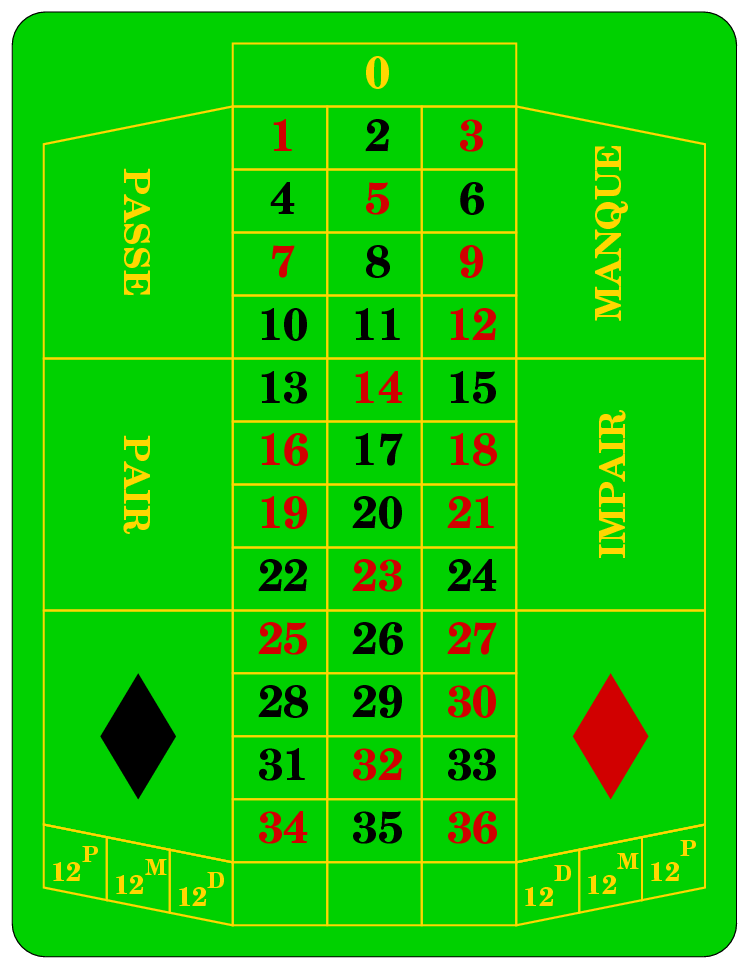
\includegraphics[width=4.5cm]{Roulette_frz.png}
  \caption{Farben der Zahlen beim Roulette}
\end{wrapfigure}
Beim Roulette gibt es 37 Nummernf\"acher mit den Nummern 0 bis 36. Die 0 hat die Farbe gr\"un, die anderen Zahlen sind rot oder schwarz wie in Abbildung 1 dargestellt. Fridolina setzt immer 1 Euro auf rot. Wie viel gewinnt oder verliert Fridolina durschnittlich pro Spiel? 

Lösung: Wir modellieren das Problem zun\"achst als ein \rule{2cm}{.4pt}-Experiment, bei dem jedes \rule{3cm}{.4pt} $\omega$ in der \rule{3cm}{.4pt} $\Omega$ diesselbe Wahrscheinlichkeit hat.
Also: $$\Omega = \rule{6cm}{.4pt} $$
$X$ sei nun eine Zufallsvariable, die den Gewinn in Euro bezeichnet. Eine Zufallsvariable ist immer eine Abbildung von $\Omega$ in die reellen Zahlen. Bei uns kann $X$ nur die Werte \rule{1cm}{.4pt} oder \rule{1cm}{.4pt} annnehmen. Zum Beispiel entnehmen wir Abbildung 1, dass für das Ergebnis $\omega = 5$ gilt: $X\left( \omega \right) = 1$. Und für $\omega = 15$ gilt: $X\left( \omega \right) = -1$.

\textbf{Aufgabe 1:} Was ist $X\left( 16 \right)$, $X\left( 17 \right)$ und $X\left( 18 \right)$ ?
\vspace{1cm}

Wie viel gewinnt Fridolina nun durchschnittlich pro Runde? Um diese Frage zu beantworten, stellen wir uns vor, dass Fridolina dass Spiel sehr oft, d.h. zum Beispiel, $n=1.000.000$-mal spielen würde. Dabei wäre es dann zu folgendem Ergebnis gekommen:
\begin{center}
\renewcommand{\arraystretch}{1.7}
 \begin{tabular}{|c|c|c|}
 \hline
 Ereignis & $X=1$ & $X=-1$ \\
 \hline
 Anzahl & $486.000$ & $514.000$ \\
 \hline
 \end{tabular}
 \end{center}
 \textbf{Aufgabe 2:} Berechnen Sie in diesem Fall den durschschnittlichen Gewinn $\overline{x}$ pro Spielrunde!
\vspace{2cm}



$h_n\left(X=1\right) = \rule{3cm}{.4pt}$ ist die \rule{3cm}{.4pt} H\"aufigkeit des Ereignisses $X=1$. Wenn wir $\overline{x}$ nun mittels der \rule{3cm}{.4pt} Häufigkeiten schreiben, ergibt sich:
$$ \rule{8cm}{.4pt} $$
Die Wahrscheinlichkeit eines Ereignisses ist die \rule{3cm}{.4pt} H\"aufigkeit bei \rule{3cm}{.4pt} großer Stichprobenl\"ange $n$. In Formeln: $ \lim\limits_{n \rightarrow \infty}{h_n\left(X=1\right)} = \rule{2cm}{.4pt} $.
Der Erwartungswert von $X$ ist gleich $\overline{x}$ bei \rule{3cm}{.4pt} großer Stichprobenl\"ange $n$. D.h.

$$ E\left[ X \right] = \rule{8cm}{.4pt}$$.

\textbf{Aufgabe 3:} Berechnen Sie nun den Erwartungswert von $X$!

\end{document}
